Lenses keep two similar pieces of data consistent; as either one evolves,
the lens finds analogous evolutions for the other. However, current lenses
don't generalize smoothly to more than two pieces of data. Spreadsheets
manage many pieces (cells) of data that are related to each other, but they
are generally unidirectional: some cells are special automatically-updated
cells, and the values in these cells are always computed by the system and
cannot be changed by the user. Constraint propagation systems generalize
spreadsheets to be many-directional when possible. However, current systems
do not use old states of the system to guide the computation of new states;
any system state which satisfies the given constraints is allowed.

% TODO: Benjamin says: ``This intro is going to get some more polishing,
% right?''

The goal of the hyperlenses project is to merge the three systems, giving a
way of maintaining constraints between many pieces of data that, when given
an update to some part of the system, finds an ``analogous'' update to the
rest of the system. Below we discuss criteria on which the success of the
hyperlenses project can be judged.

In typical constraint propagation systems, there are variables and
constraints. Constraints may involve any number of variables, and are simply
relations on valuations of those variables. In the following, many of the
relations we care about will be of the form
\[\{(x_1,\ldots,x_m,y_1,\ldots,y_n) \mid f(\overline x) = g(\overline y)\}\]
and so we will simply write these as
$f(\overline x) = g(\overline y)$
when it is clear from context that a relation is expected.

\section{Simple example}
A user might draw up a vacation expenditures spreadsheet that looks like
this:

\begin{tabular}[h]{lrrrr}
    Day     & Travel    & Lodging   & Food  & Total \\
    1       & 750       & 120       & 45    & 915   \\
    2       & 30        & 120       & 18    & 168   \\
    3       & 0         & 120       & 150   & 270   \\
    4       & 15        & 120       & 30    & 165   \\
    5       & 750       & 0         & 15    & 765   \\
    Total   & 1545      & 480       & 258   & 2283  \\
\end{tabular}

Along with the table, we would expect to see some constraints like
\begin{align*}
    \mathrm{Travel}_\mathrm{Total} &=
    \mathrm{Travel}_1+\mathrm{Travel}_2+\mathrm{Travel}_3+\mathrm{Travel}_4+\mathrm{Travel}_5
    \\
    \mathrm{Total}_1 &= \mathrm{Travel_1}+\mathrm{Lodging}_1+\mathrm{Food}_1
\end{align*}
and so on, with ten constraints in all (one each for days 1, 2, 3, 4, 5, and
Total, and one each for categories Travel, Lodging, Food, and Total). Here
are some things a user might want to do with this setup:
\begin{itemize}
    % TODO: about this \item, Benjamin says: ``?''
    \item The user might go on another vacation, and want to make an
        estimate of how much he spent on food given his credit card balance
        at the end of the trip. To do this, he might update
        $\mathrm{Total}_\mathrm{Total}$ to his balance and look in the
        $\mathrm{Food}_\mathrm{Total}$ cell to get a guess.
    \item The user might like to plan a vacation to a certain
        location with a certain budget; then he could fix the
        $\mathrm{Total}_\mathrm{Total}$ cell and update the travel prices
        for the first and last day's plane tickets to get an estimate of how
        much he can spend on the various other days and categories while
        staying in his budget.
    \item Perhaps the user discovers that he is missing a category for
        entertainment and wants to add a new column, initially populated
        with zeros. He did not keep careful track of his daily spending for
        this on the last vacation, but he knows that in total he spent about
        \$800 on entertainment, so he updates the new
        $\mathrm{Entertainment}_\mathrm{Total}$ cell to 800.
        % TODO: Benjamin says: ``And then...?
        %
        % Overall, it seems like these use cases could be crisper.``
\end{itemize}

\section{Goal statement}
\label{sec:goal_statement}
{\bf A hyperlens should be a generalization of both lenses and spreadsheets that
supports high-level planning.}

Hyperlenses should generalize lenses. It should be true that there is a
behavior-preserving embedding of asymmetric, state-based lenses: that is, we
can identify two variables in the hyperlens system whose values correspond
to states of the asymmetric lens' two repositories, and the values in the
hyperlens system evolve in the same way they would evolve when running the
lens itself. Moreover, we demand that there be a ``hyperlens composition''
that preserves this property: the embedding of a composition of lenses is
the composition of their embeddings.

A stretch goal is to generalize symmetric, state-based lenses in a similar
way, and again to find a composition operator (potentially different from
the previous one) that corresponds to symmetric lens composition.

Hyperlenses should generalize spreadsheets. It is unreasonable to demand
that the hyperlens framework be capable of bidirectionalizing all
spreadsheets in a reasonable way. However, on the class of spreadsheets that
can be bidirectionalized, it should be the case that using the corresponding
hyperlens as if it were a unidirectional spreadsheet produces the same
answers as the original spreadsheet would.

A stretch goal is to generalize spreadsheets in the sense that any
spreadsheet can be expressed as a (possibly still unidirectional) hyperlens
with the same behavior.

Hyperlenses should support high-level planning. As with all bidirectional
systems, there will be some updates which can be spread through the
remainder of the system in many ways. Support for high-level planning means
that there is some holistic language (that is, which does not require
intimate knowledge of the structure of the term used to define the
hyperlens) for expressing the relative desirability of the various coherent
updates to the system. The system should then be able to compute the most
desirable update. For example, being able to request that a particular
variable be a sink for as much of the change as possible would satisfy this
requirement.

% TODO: cite a few use cases with the high-level planning we want for each
\section{Simplistic solutions}
Some particularly simple regimes have already been explored. Four such
regimes are discussed below, but it will be helpful to have a few
conventions in place first.

Fix a linearly ordered set $\Names$ of names and a universe $U$ of values.
Since we are dealing with partial functions, we will use the convention that
$a = b$ whenever both $a$ and $b$ are undefined or whenever $a$ and $b$ are
defined and identical. Likewise, $a \in b$ means that both $a$ and $b$ are
undefined or they are both defined and $a$ is a member of $b$.

\begin{definition}
    A \emph{valuation} is a finite map from $\Names$ to $U$.
\end{definition}

We generalize valuation application from names to finite sets of names using
the linear ordering on $\Names$: whenever $x_1 < \cdots < x_m$ is an
increasing chain, $f(\{x_1,\ldots,x_m\}) = (f(x_1),\ldots,f(x_m))$.

\begin{definition}
    A \emph{constraint} is a finite set $n \subset \Names$ together with a
    relation $R \subset U^{|n|}$.
\end{definition}

\begin{definition}
    A valuation $f$ \emph{satisfies} constraint $(n,R)$ when $f(n) \in R$.
\end{definition}

\begin{definition}
    The \emph{constraint system graph} induced by a set of constraints is
    the undirected bipartite graph whose nodes are drawn from $\Names$ in
    one part and constraints in the other, and which has an edge $(v,(n,R))$
    iff $v \in n$.
\end{definition}

In some systems we discuss below, each constraint will have a clear notion
of ``output'' variable. In these systems it will be convenient to also have
a directed variant of the constraint system graph.

\begin{definition}
    A \emph{pointed constraint} is a pair $(v,(n,R))$ of a constraint and a
    designated variable $v\in n$.
\end{definition}

\begin{definition}
    The \emph{directed constraint system graph} induced by a set of pointed
    constraints is a directed bipartite graph whose nodes are drawn from
    $\Names$ in one part and pointed constraints in the other. It has an
    edge from $v$ to $(v',(n,R))$ iff $v \ne v'$ and $v \in n$, and it has
    an edge from $(v',(n,R))$ to $v$ iff $v=v'$.
\end{definition}

% TODO: Benjamin says: ``We need an example to follow all this.''
\begin{definition}
    A \emph{root node} is a node in a directed graph with in-degree zero.
\end{definition}

\begin{definition}
    A node has \emph{high in-degree} if its in-degree is greater than one.
\end{definition}

In a directed constraint system graph, a root node corresponds to a name
that is not the output of any constraint.

\subsection{Spreadsheets}
One particularly simple regime is where there is a directed constraint
system graph with no cycles, no nodes with high in-degree, and edits are
made only to root nodes. This corresponds to how most well-known
spreadsheets behave. However, the restriction that you may only edit root
nodes is quite limiting: it essentially means that the system is
unidirectional.

\subsection{Tree topology}
The lens frameworks discussed in \ref{chap:finished_work} amount to having a
constraint system graph with exactly two variables and exactly one
constraint connecting them. You may only edit one of the variables at a
time. Then, to propagate the change, you spread the change from the changed
variable to the unchanged one.
%
We can take the idea of propagating change from changed variables to
untouched ones somewhat further: when the constraint system graph is a tree, an
update to a single node may be propagated through the entire graph by
treating the updated node as a root of the tree and updating the values of
nodes in topologically-sorted order.

We leave the discussion here short because this solution is completely
subsumed by the solution in Section~\ref{sec:nonassociative_composition}.

\subsection{Linear constraints}
\label{sec:linear_constraints}
Consider this simple, non-tree-structured spreadsheet:
\begin{align*}
    tax &= 0.08*base \\
    total &= base + tax
\end{align*}
Despite the mildly interesting structure of the constraint system graph, it
is still definitely possible to bidirectionalize this spreadsheet.

Suppose each constraint in the spreadsheet is \emph{linear}, that is, has
the form
\[x = b+\sum_ic_iy_i\]
for some constants $b$ and $\overline c$. Additionally, we take the topological
constraints that the directed constraint system graph has no (directed)
cycles or nodes with high in-degree. (Note that the two-equation spreadsheet
above has cycles in its constraint system graph but not its directed
constraint system graph.)

Under these assumptions, a simple argument shows that, given a cell in the
spreadsheet, we can write an affine formula which maps the values of root
cells to the value of the given cell. The argument goes by induction on the
length of the longest path from a root cell to the given one, and proceeds
by substituting in affine formulas for each non-root variable at each step.
In fact, we can go a step farther: we can write affine transformations from
root cells to any set of cells. If we manage to give a characterization of
when these affine transformations can be bidirectionalized, then we will
have given an account of how to handle the multi-update problem and relax
the simple structure requirement in the parts of the spreadsheet where only
affine formulae are used.

Thus, we can now frame our problem in another way: what is the right way to
bidirectionalize an affine transformation? Accordingly, we will now step
away from spreadsheets and frame our discussion in linear algebra terms.

A function $\aget \in \R^m \to \R^n$ is affine exactly when there is a matrix
$M$ of dimension $n \times m$ and vector $\mathbf b \in \R^n$ such that $\aget(\x) =
M\x +\mathbf b$.  Affine functions are surjective (and hence bidirectionalizable)
just when $M$ has rank $n$, so we assume this. When $m=n$, $f$ is a
bijection. The put function in this case is particularly boring, because it
ignores the original source:
\[\aput(\x,\y) = M^{-1}(\y-\mathbf b)\]
The more interesting case is when $m>n$, and where each $\y$ is therefore
the image of a nontrivial subspace of $\R^m$. There are many heuristics one
may choose to identify a particular point in this subspace; we choose the
specification:
\[\aput(\x,\y) = \argmin{\x',\aget(\x')=\y}||\x' - \x||\]

\begin{lemma}
    There exists an $m \times n$ matrix $P$ such that
    \[\aput(\x,\y) = \x + P(\y - \aget(\x))\]
    satisfies the specification above.
\end{lemma}
\emph{Proof sketch.} The intuition is that we wish to move as little as
possible in source-space to match the move in target-space. This can be
achieved by minimizing how far we move in the null space of $M$, since
(exactly) these motions result in no motion in target-space.
% TODO: Benjamin says: ``Remind what the null space is?''

Take a basis $\{\x_1,\ldots,\x_{m-n}\}$ for the null space of $M$. Then
we will take:
\begin{align*}
    B &= \left[\begin{array}{c}
            \x_1\transpose \\
            \vdots \\
            \x_{m-n}\transpose
        \end{array}\right] \\
    P &= \left[\begin{array}{c}
            M \\
            B
        \end{array}\right]^{-1}
        \left[\begin{array}{c}
            I_n \\
            \mathbf 0_{m-n,n}
        \end{array}\right] \\
\end{align*}
Turning the sketch into a proof involves arguing three things: that the
square matrix in the definition of $P$ is invertible; that $P$ produces a
put function that roundtrips; and that the put function produced by $P$
produces minimal changes. The definition above was crafted so that (assuming
for the moment that $P$ exists) we have $MP = I$, which is used to show the
roundtrip property, and $BP = \mathbf 0$, which is used to show minimality.

% TODO: finish this proof and replace the above sketch, maybe

%\begin{proof}
%    The intuition is that we wish to move as little as possible in
%    source-space to match the move in target-space. This can be achieved by
%    minimizing how far we move in the null space of $M$, since (exactly)
%    these motions result in no motion in target-space.
%
%    Take a basis $\{\x_1,\ldots,\x_{m-n}\}$ for the null space of $M$. Then
%    we will take:
%    \begin{align*}
%        B &= \left[\begin{array}{c}
%                \x_1\transpose \\
%                \vdots \\
%                \x_{m-n}\transpose
%            \end{array}\right] \\
%        P &= \left[\begin{array}{c}
%                M \\
%                B
%            \end{array}\right]^{-1}
%            \left[\begin{array}{c}
%                I_n \\
%                \mathbf 0_{m-n,n}
%            \end{array}\right] \\
%    \end{align*}
%    We must now argue three things: that the square matrix in the definition
%    of $P$ is invertible; that $P$ produces a put function that roundtrips;
%    and that the put function produced by $P$ produces minimal changes. The
%    definition above was crafted so that (assuming for the moment that $P$
%    exists) we have $MP = I$, which is used to show the roundtrip property,
%    and $BP = \mathbf 0$, which is used to show minimality.
%
%    invertible: (TODO)
%
%    roundtrip:
%        \begin{align*}
%            \aget(\aput(\x,\y))
%                &= M(\x+P(\y-M\x-\mathbf b))+\mathbf b & \mbox{definition of }\aget,\aput \\
%                &= MP\y + M\x + \mathbf b - MP(M\x + \mathbf b) & \mbox{rearranging terms} \\
%                &= \y & MP=I
%        \end{align*}
%
%    minimal: (TODO)
%\end{proof}

\subsection{Biased graph combination}
\label{sec:nonassociative_composition}
In the three previous solutions, we have carefully restricted the allowed
graph topologies and valuation updates so that there is at most one best
strategy for reinstating constraints. This skirts one of the major goals of
the hyperlens project: developing tools that embrace ambiguous updates and
provide tools for disambiguating. In this section, we will explore a setting
with some slight ambiguity and a way to give programmer control. We will
also allow multi-update, and give a type system describing statically
solvable updates. The high-level idea is to combine two small constraints on
variable sets $S$ and $T$ into a single large constraint on variable set $S
\cup T$ in a biased way: the programmer designates one of the two
constraints as special, and whenever an update could be resolved by
resolving the two constraints in either order, we choose to resolve the
special constraint first.

Consider the spreadsheet given by these two schematic constraints:
\begin{align*}
    o_1 &= f(i_1, i_2) \\
    o_2 &= g(i_1, i_2)
\end{align*}
Given an update to $i_1$, it may be possible to resolve these two
constraints in either of the following two ways:
\begin{itemize}
    \item First, update $i_2$ and $o_1$ to restore the $f$ constraint.
        Then, update $o_2$ without modifying $i_1$ or $i_2$ (so as not to
        disrupt the already-restored $f$ constraint) to restore the $g$
        constraint.
    \item Symmetrically, first update $i_2$ and $o_2$ to restore the $g$
        constraint, then update $o_1$ without modifying $i_1$ or $i_2$ to
        restore the $f$ constraint.
\end{itemize}
It is perfectly reasonable for these two plans to choose different updated
values for $i_2$. One way to resolve the tie is to give either $f$ or $g$
higher priority.

Let us call the objects of this simple solution \emph{multiway lenses}. We
will give a definition, show how to combine multiway lenses (so that e.g.
the above example would be the combination of one multiway lens for the $f$
constraint and one for the $g$ constraint), and briefly discuss some
limitations of this approach.

\begin{definition}
    Given $N\subset\Names$, a \emph{multiway lens} $\ell \in \mlens N$
    is a triple $(\danger,\mput,K)$ where
    \begin{itemize}
        \item $\danger \in 2^{2^N}$ is a predicate on sets of names called the \emph{danger
            zone} of $\ell$,
        \item $\mput \in 2^N \to (N \to U) \to (N \to U)$ is an update
            function which takes a set of names and a valuation on $N$ and
            produces another valuation, and
        \item $K$ is an invariant expressed as a predicate on valuations on
            $N$.
    \end{itemize}
\end{definition}

The danger zone will be our ``type system'': updates to sets of variables
that are in the danger zone are statically unsolvable. The first argument to
the $\mput$ function should be read as marking which variables have been
updated. There are some well-formedness conditions on multiway lenses.
First, we will want an analog of the lens framework's roundtrip laws. We
will also ask that danger zones be sensible in the sense that updating more
variables does not make the constraint system more solvable, and that the
$\mput$ function restrain itself to modifying parts of the valuation that
are not inputs.

% TODO: define upwards-closed
\begin{definition}
    A multiway lens $\ell$ is \emph{well-formed} when it satisfies the
    following laws:
    \begin{itemize}
        \item $\mput(i,f) \in K$ whenever $i \notin \danger$
        \item $\mput(i,f) = f$ whenever $f \in K$
        \item $\danger$ is upwards-closed
        \item $\left.\mput(i,f)\right|_i = \left.f\right|_i$
    \end{itemize}
\end{definition}

In the definition of multiway lens composition below, it will be convenient
to extend $\mput$ functions so that they act on valuations that cover extra
variables by leaving the extra variables' values unchanged.
\begin{definition}
    Suppose we have $N \subset M \subset \Names$, a lens $k \in \mlens{N}$,
    a set of names $i \subset M$, and $f$ is a valuation on $M$. Then
    $\focus(k,i,f)$ is a valuation on $M$:
    \begin{align*}
        \focus(k,i,f)(x) &= \cond{
            k.\mput(i \cap N,f|_N)(x) & x \in N \\
            f(x) & x \notin N
        }
    \end{align*}
\end{definition}

\begin{definition}
    Suppose $k \in \mlens{N_k}$ and $\ell \in \mlens{N_\ell}$ and let $S =
    N_k \cap N_\ell$ be the set of shared variables. Then the composition
    $k\mid\ell \in \mlens{N_k \cup N_\ell}$ of $k$ and $\ell$ has:
    \begin{align*}
        \danger &= k.\danger \cup \ell.\danger \cup
            \{(d_k \cup d_\ell) \setminus S
            \mid d_k \in k.\danger, d_\ell \in \ell.\danger\} \\
        \mput(i) &= \cond{
            \focus(\ell,i\cup S) \circ \focus(k,i)
                & i \notin k.\danger \land i\cup S \notin \ell.\danger \\
            \focus(k,i\cup S) \circ \focus(\ell,i)
                & \mbox{otherwise}
            } \\
        K(f) &= k.K(f|_{N_k}) \land \ell.K(f|_{N_\ell})
    \end{align*}
\end{definition}

\begin{lemma}
    $k\mid\ell$ is well-formed whenever $k$ and $\ell$ are.
\end{lemma}

In the definition of $(k\mid\ell).\mput$, there are two clauses
corresponding to running $k$ first and running $\ell$ first, respectively.
The side condition on the first clause---$i \notin k.\danger \land i \cup S
\notin \ell.\danger$---itself has two parts that amount to
checking that we can safely run $k.\mput$ and that we can treat all of the
outputs of $k.\mput$ as inputs when running $\ell.\mput$, respectively. The
bias alluded to above arises from the fact that the second clause is active
only when the first clause fails; in cases where it is safe to run either
$k$ or $\ell$ first, we arbitrarily choose to run $k$ first.

The danger zone defined for composition ensures that it is safe to run one
of the two sub-multiway lenses first. Returning to our example, suppose the
base lenses $\ell_f$ and $\ell_g$ for the $f$ and $g$ constraints had danger
zones saying only that we can not update all three variables involved at
once, that is:
\begin{align*}
    \ell_f.\danger &= \{\{i_1,i_2,o_1\}\} \\
    \ell_g.\danger &= \{\{i_1,i_2,o_2\}\}
\end{align*}
Then, the danger zone for $\ell_f \mid \ell_g$ would be
\[\{\{i_1,i_2,o_1\},\{i_1,i_2,o_2\},\{o_1,o_2\}\}\]
which says that an update is dangerous if it's dangerous for either of the
sub-multiway lenses \emph{or} if it changes both outputs at once. In the
latter case, it would not be safe to run either sub-multiway lens first,
since this would over-constrain the other sub-multiway lens.

Multiway lenses are an attractively simple formalism, but they do have some
serious drawbacks. For example, it is clear by design that composition is
not commutative. A more subtle and important failing is that composition is
not \emph{associative}. This is because the composition discussed here
treats its components as black boxes: it will run each of its components as
a chunk. As a result, we find that $(k \mid \ell) \mid m$ will always run
$m$ either first or last---never in between $k$ and $\ell$---and will
therefore sometimes fail where $k \mid (\ell \mid m)$ can succeed by
choosing one of these $m$-in-the-middle orderings.

%We can also define renaming on names in the lens' domain.
%\begin{definition}
%    Given $\ell \in \mlens N$ and two names $V \in N$ and $W \notin N$, we can
%    give the renaming $\ell[W/V]$:
%    \begin{align*}
%        \danger &= \{d[W/V] \mid d \in \ell.\danger\} \\
%        \mput(i,f) &= \ell.\mput(i[V/W], f[V/W])[W/V] \\
%        K(f) &= \ell.K(f[V/W])
%    \end{align*}
%\end{definition}
%
%\subsection{Primitive Lenses}
%\begin{definition}
%    The identity lens $\id : \mlens{\{A,B\}}$ is defined as follows:
%    \begin{align*}
%        \danger &= \{\{A,B\}\} \\
%        \mput(\{A\},f) &= f[B \mapsto f(A)] \\
%        \mput(\{B\},f) &= f[A \mapsto f(B)] \\
%        \mput(\{\},f) &= f[A \mapsto f(B)] \\
%        K(f) &= f(A) == f(B)
%    \end{align*}
%\end{definition}
%
%For a value $u \in U$, we define a constant lens which enforces the
%invariant that a cell is always equal to $u$.
%
%\begin{definition}
%    If $u \in U$ then the constant lens
%    $\const(u) : \mlens{\{A\}}$ is defined as:
%    \begin{align*}
%        \danger &= A \\
%        \mput(i,f) &= \lambda v. u \\
%        K(f) &= f(A) == u
%    \end{align*}
%\end{definition}
%
%Conjecture: all these lenses and combinators are well-behaved.

\section{Design axes}
\label{sec:design_axes}
A full solution could reasonably build on either the restrictive constraints
of the linear solution
or the restrictive topology of the tree-structured solution. Because it seems
difficult to extend the restrictive constraints solution sufficiently to
achieve our top-level goal of embedding all asymmetric, state-based lenses,
the approach of extending the restrictive topology solution seems more
promising. Below, we discuss some of the difficulties that should be addressed
by a successful generalization.

There is a distinction between the dynamic and static semantics of a
constraint system graph. Unless specified otherwise, all discussion is of
the static semantics.
\begin{definition} Semantics:
    \begin{description}
        \item[Dynamically ambiguous] means the current set of constraints and
            requested updates have multiple satisfying valuations.
        \item[Dynamically unsolvable] means the current set of constraints and
            requested updates have no satisfying valuations.
            % TODO: these definitions of statically ambiguous and statically
            % unsolvable are awful
        \item[Statically ambiguous] means there is a set of requested updates
            and a set of constraints whose graph is the current one which is
            dynamically ambiguous.
        \item[Statically unsolvable] means there is a set of requested updates
            and a set of constraints whose graph is the current one which is
            dynamically unsolvable.
    \end{description}
\end{definition}

\subsection{Sources of ambiguity}
\subsubsection{Intra-constraint ambiguity}
Consider the very simple constraint system which has only one constraint, $z
= x+y$. Giving a value for $z$ gives us a classical ``underconstrained
system'': there are infinitely many choices for $x$ and $y$ that satisfy
this constraint. For example, we might choose to keep $y$ and only update
$x$, we might choose to increase $x$ and $y$ by the same summand, we might
ignore the old values of $x$ and $y$ altogether and make them both be
particular fractions of $z$, we might attempt to preserve the product $x*y$,
etc. In our simple example, when we update the grand total, one reasonable
choice would be to scale all the summands by the same factor the grand total
was scaled by.

More abstractly, we might wish to have some runtime control over how
constraint solutions are being chosen in case there is ambiguity.

\begin{desiderata}
    Have programmer-level control over the resolution of individual
    constraints.
\end{desiderata}
\begin{desiderata}
    Have high-level control over the resolution of individual constraints.
\end{desiderata}

\subsubsection{Cycles and inter-constraint ambiguity}
Above, we discussed the possibility of constraint system graphs with cycles
in them. We observed that in such situations, it may be that no ordering of
the constraints' methods may result in a consistent state; however, there
are also situations where many orderings each result in a consistent state
-- and indeed, the chosen consistent states may even differ. As a very
simple example, consider this system that has some seemingly redundant
variables:
\begin{align*}
    z_1 &= x+y \\
    z_2 &= x+y
\end{align*}
We will assume that each constraint either allows us to update $z_i$ alone
given $x$ and $y$ or allows us to update $z_i$ and $y$ together. The first
constraint uses the update policy
\[(z_1',y') = \left(z_1 + \frac{x'-x}2, y - \frac{x'-x}2\right)\]
which spreads half the change to each variable, while the second constraint
uses the update policy
\[(z_2',y') = \left(z_2 + \frac{x'-x}3, y - \frac{2(x'-x)}3\right)\]
which spreads only a third of the change to $z_1$ and the rest to $y$.
% TODO: picture

Suppose we start from the all-zero valuation and then update $x$ to $6$.
There are (at least) two reasonable update plans that guarantee consistency:
update $z_1$ and $y$ together to $3$ and $-3$, respectively, then update
$z_2$ to $3$, or the symmetric plan that updates $z_2$ and $y$ together to
$2$ and $-4$, then updates $z_1$ to $2$.

\begin{desiderata}
    Provide high-level control over ambiguous cycles.
\end{desiderata}

\subsection{Sources of insolubility}
\subsubsection{Cycles}
Suppose we have three variables, $x$, and $y$, and $z$, and three
constraints, one on each pair of variables. We will allow ourselves to
assume we also have a collection of methods for each individual constraint
that can take an update to one of the variables and produce a value of the
other variable that satisfies the constraint. The question now becomes: can
we take an update to one variable, say, $x$, and produce updates to the
other two that reinstate all three constraints?
% TODO: Benjamin says: ``Overall, the document needs a bunch of high-level
% signposting. The reader needs to understand why they are being told all
% this stuff, not just the stuff...''

The naive approach, where we compute $y$ from our assumed method that
reinstates the $\{x,y\}$ constraint and $z$ from our assumed method that
reinstates the $\{x,z\}$ constraint doesn't necessarily work, since there is
no guarantee that the $y$ and $z$ computed this way satisfy the $\{y,z\}$
constraint.

Consider our simple example above: there are two ``paths'' in the constraint
graph from the $\mathrm{Total}_\mathrm{Total}$ node to the
$\mathrm{Travel}_1$ node, namely via $\mathrm{Total}_1$ and via
$\mathrm{Travel}_\mathrm{Total}$. What we would be asking for is a guarantee
that, for example, the way we choose to spread an update over the category
totals and thereafter over the individual cells is compatible with the way
we choose to spread an update over the day totals and thereafter over the
individual cells. In the case of our simple example, we could certainly
achieve this using arithmetic facts, but in more complicated examples the
way forward is less clear.

\begin{desiderata}
    Handle dynamically solvable cycles.
\end{desiderata}

\subsubsection{Multiple update}
Many constraint propagation systems support the update of multiple variables
simultaneously. As discussed in our simple running example, making a
vacation plan on a budget might involve setting the grand total and the
travel costs all at once. This is distinct from setting them one at a time,
since we want the system to guarantee that all three values can coexist,
whereas when we set them one at a time each update may disrupt the values of
the other two.

\begin{desiderata}
    Identify solvable multiple updates.
\end{desiderata}

\subsection{Other difficulties}
\subsubsection{Algebraic structure}
Experience with programming in other lens languages has shown that
sequential composition is a key feature for modularity. Hyperlens
composition may not necessarily be sequential, but there should be some
tools for developing hyperlenses in a modular way. For this to make sense,
we expect that the programmer will wish for composition to be associative
(so that how modules are combined does not matter) and may even wish for
composition to be commutative (so that the order modules are defined does
not matter).
\begin{desiderata}
    Provide an associative, commutative composition operation.
\end{desiderata}
\subsubsection{Efficiency}
We would like the hyperlens project to produce a framework that is usable
for very large data sets, even when there is a lot of ambiguity. It is very
easy to design constraint system graph topologies where certain updates
produce an enormous number of reasonable full update plans; a good solution
to the problem should be able to not only choose one of these plans, but
also do so in an efficient way.
\begin{desiderata}
    Select an update plan in polynomial time in the size of the hyperlens.
\end{desiderata}
\begin{desiderata}
    Reinstate coherence in a single pass: for each constraint, execute one
    method at most once.
\end{desiderata}
\subsubsection{Syntax}
Any sensible formalism can be instantiated; for example, a sensible
hyperlens formalism should include operations that correspond to some of the
basic computations done with spreadsheets: some arithmetic, perhaps some
simple string operations, aggregations, composition, and so on.
\begin{desiderata}
    Provide a syntax for basic spreadsheet programming.
\end{desiderata}

\subsubsection{Inter-constraint coordination}
It would be nice if the hyperlens associated with
\begin{align*}
    x &= a+b \\
    y &= x+c
\end{align*}
behaved ``similarly'' to the hyperlens associated with
\begin{align*}
    x &= b+c \\
    y &= a+x
\end{align*}
in the sense that an update to $y$ in either system resulted in the same
updates to $a$, $b$, and $c$. This is nice from a language design point of
view because it means you need not introduce separate $+$ functions for each
arity, and is nice from a usability point of view because it means that
there is no price to pay for modularity: you can split up your code into
whatever units make sense to you and get the same program out.

\begin{desiderata}
    Allow constraints to interact during system update.
\end{desiderata}
% TODO: Benjamin says: ``Some discussion is needed about (a) what's been
% done and learned so far, and (b) what, concretely, you plan to do, and
% what you expect the result to be.''
\section{Timeline}
\label{sec:timeline}
Currently, the most promising approach is to use local constraint
propagation-style update planning, but add some features to give programmer
control of constraint resolution order in situations where the order is
ambiguous. One major unfinished piece of work is inventing and evaluating
such schemes for providing programmer control. I expect there to be a
tradeoff involved between flexibility (how much control the programmer has)
and simplicity (how expert the programmer must be to achieve his goals).

Having simple, high-level control is a major goal of the project;
nevertheless, I propose to begin with a serious investigation of very
flexible, low-level control schemes, with the hopes that (1) a solid
understanding of the behavior of low-level controls will guide the design of
high-level schemes, and (2) that low-level schemes may serve as a
``compilation target'' for high-level schemes---and an escape hatch when the
less flexible schemes produce undesirable update plans.

The other major unfinished work involves investigating how to incorporate
high quality, special-purpose constraint solvers. For example, the linear
constraint solver proposed in \ref{sec:linear_constraints} has many
desirable properties, and would be a convenient component in a larger
system; as would dynamic solvers for statically unsolvable cycles.

I propose the following timings:
\begin{itemize}
    \item Low-level control schemes: 2 months
    \item High-level control schemes: 1 month
    \item Incorporating black boxes for linear and cyclic solvers: 1 month
    \item Extending the linear solver to nonlinear functions: 2 months
    \item Defense writing: 3 months
\end{itemize}
This proposed timeline is also shown in Figure~\ref{fig:timeline}, which
includes some possible publication targets as well as one month of slack
time for preparing publications.
\begin{figure}
    \centering
    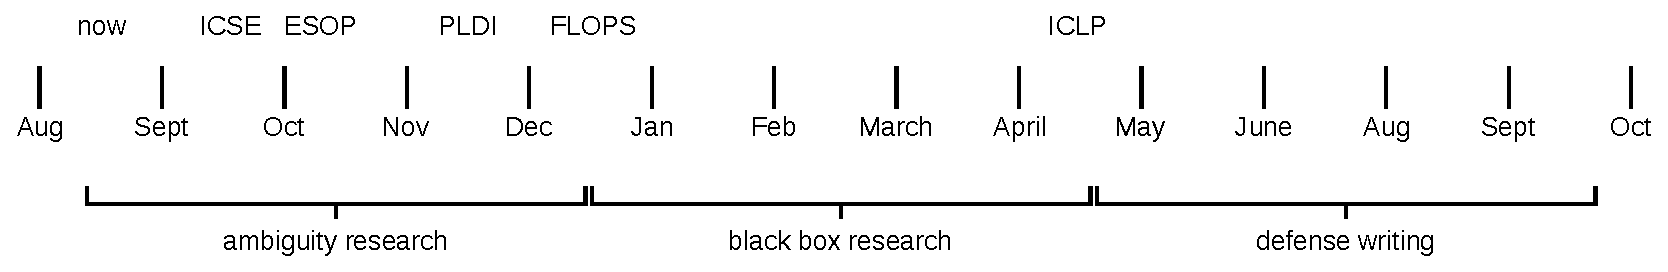
\includegraphics[scale=0.6]{timeline.pdf}
    \caption{Proposed research timeline}
    \label{fig:timeline}
\end{figure}
